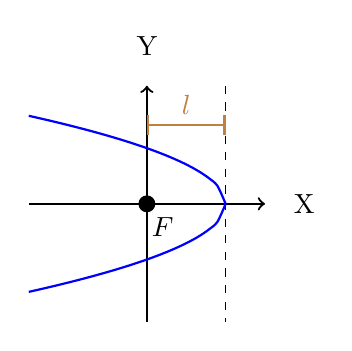
\begin{tikzpicture}

\node at (-1,0) {};
\draw [->, thick] (-2.5,0) -- (0.5,0);
\draw  [<-, thick](-1,1.5) -- (-1,-1.5);
\draw  [fill](-1,0) node (v1) {} circle (0.1);

\draw [dashed] (0,1.5) -- (0,-1.5);
\draw [|-|, thick, brown] (0,1) -- (-1,1) node [midway, above]{$l$};
\node at (1,0) {X};
\node at (-1,2) {Y};
\node at (-0.8,-0.3) {$F$};
\draw[thick, scale=0.5,domain=-5:0,smooth,variable=\x,blue] plot (\x,{sqrt(sqrt(\x*\x))});
\draw[thick, scale=0.5,domain=-5:0,smooth,variable=\x,blue] plot (\x,{-sqrt(sqrt(\x*\x))});
\end{tikzpicture}